\chapterf{Detector de batimentos cardíacos para a \textit{Nintendo Switch}}
\label{chap:bpm}

\section{Introdução}

Como tarefa pré-final, foi realizada a missão de experimentar desenvolvimentos para consolas de jogos, tendo-se a ideia de fazer um detetor de batimentos cardíacos
para a \gls{switch} e um jogo com ele designado de \textit{DMS}. Para este projeto, o único requisito era o de detetar os batimentos cardíacos de alguém com o polegar no sensor.

\section{Nintendo Switch}

A \gls{switch} (\cref{fig:switch}) é uma consola de jogos de vídeo híbrida produzida pela empresa \textit{Nintendo} com várias funcionalidades inovadoras no mercado, aspeto que caracteriza esta bem conhecida empresa.

Existem várias funcionalidades nesta consola não muito comuns noutras, como por exemplo dois comandos removíveis nas laterais, designados \textit{Joy-Cons}, podendo ser usados como comandos individuais ou como um só em conjunto.

Em ambos existem botões que se espelham um ao outro na sua quase totalidade, exceto alguns botões com funções especiais para servirem de comandos individuais quando necessário. Ambos têm um giroscópio e um acelerómetro para rastrearem movimentos; existe um \acrfull{nfc} no \textit{Joy-Con} esquerdo e um sensor de \acrshort{ir} no lado direito, este ultimo é aquele que vai ser utilizado para o \textit{DMS}.

\begin{figure}
  \centering
  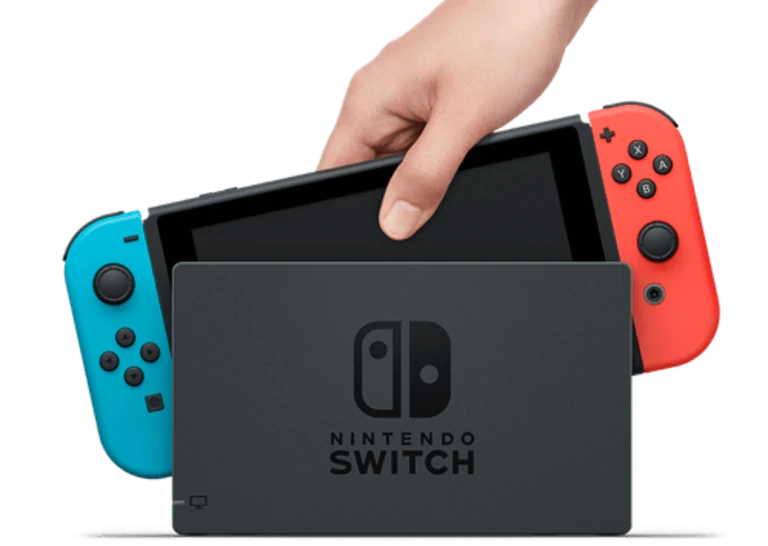
\includegraphics[width=0.9\textwidth]{switch}
  \caption{\gls{switch} \cite{switch_info}}
  \label{fig:switch}
\end{figure}



\section{DMS}

O \textit{DMS} é um jogo, desenvolvido pela \textit{Nerd Monkeys}, cujo o objetivo é o de um jogador, que esteja a segurar num \textit{Joy-Con} direito com o polegar em cima do sensor (ver \cref{fig:switch_irsensor}), tentar manter a calma enquanto outros jogadores tentam aumentar o ritmo cardíaco do outro jogador. Isto pode ser conseguido da forma que acharem mais apropriada, com historias ou mecanismos que assustem ou destabilizem o outro jogador (ex: fazer cócegas).

No contexto do jogo, o estagiário ficou responsável por fazer o detetor de batimentos cardíacos de forma a tornar esta ideia possível.

\newpage
\section{Sensor de IR}

\begin{wrapfigure}{R}{5cm}
  \centering
  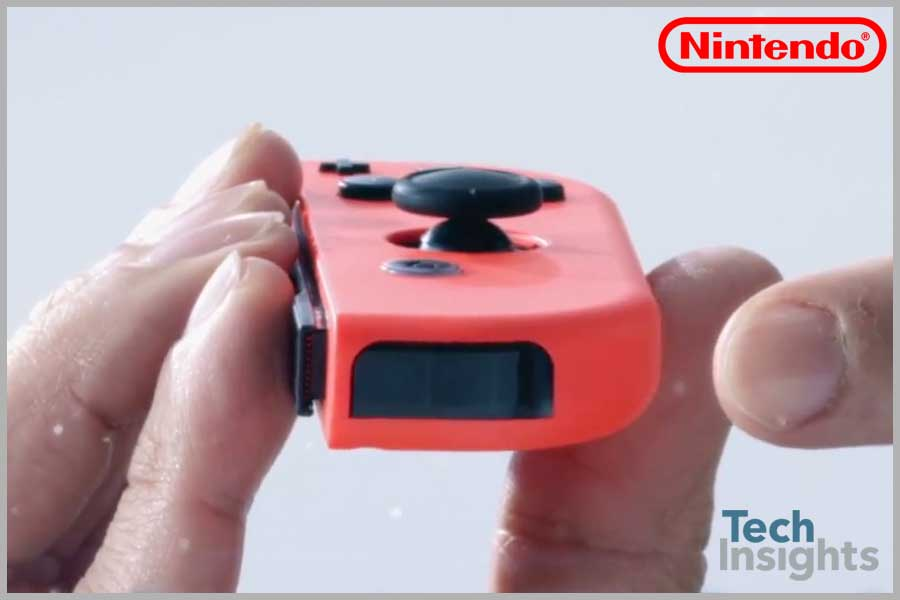
\includegraphics[width=5cm]{switch_irsensor.png}
  \caption{\acrshort{ir} \textit{Sensor} da \gls{switch} \cite{switch_irsensor_source}}
  \label{fig:switch_irsensor}

\end{wrapfigure}


O \textit{input} do sensor de \acrshort{ir} pode ser facilmente acedido por uma aplicação ou biblioteca na consola, de varias formas possíveis.

Existem várias formas de usar o sensor mas a forma mais conveniente é detetar a intensidade da luz recebida, o que pode ser usado para detetar a quantidade de oxigénio no sangue que passa no polegar. O tempo que demora entre a intensidade de subir e descer pode ser vista como o tempo de um batimento, com este tempo pode-se calcular os batimentos por minuto.

\section{Arquitetura}

Pode-se observar na \cref{fig:bpm_arch} a arquitetura do projeto, que este é desenvolvido de forma independente do jogo. O jogo só necessita de incluir a biblioteca e chamar a função para atualizar os dados, recomenda-se que esta seja chamada 60 vezes por segundo ou numa frequência superior para uma melhor deteção do valor.

\begin{figure}[H]
  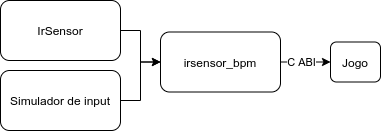
\includegraphics{batimentos}
  \caption{Arquitetura do sensor de batimentos cardíacos}
  \label{fig:bpm_arch}

\end{figure}

\newpage
\section{Tecnologias e ferramentas usadas}

Para o desenvolvimento desta biblioteca utilizou-se as ferramentas referidas na \cref{tab:bpm_software}.

\begin{table}[H]
  \centering
  \begin{tabularx}{\linewidth}{lCC}
    \multicolumn{1}{c}{\textbf{Nome}}                                       &
    \multicolumn{1}{c}{\textbf{Descrição}}                                  &
    \multicolumn{1}{c}{\textbf{Utilização no projeto}}
    \tabularnewline \tabularnewline
    C++                                                                     &
    Uma linguagem de programação compilada multi-paradigma e de uso geral.  &
    Linguagem usada para programar a biblioteca.
    \tabularnewline \midrule
    \textit{Nintendo SDK}                                                   &
    Ferramentas usadas para desenvolver para sistemas da \textit{Nintendo}. &
    Usadas para acessar as \acrshortpl{api} da \gls{switch} e compilar a biblioteca.
    \tabularnewline \midrule
    \textit{Visual Studio}                                                  &
    Um \acrshort{ide} criado pela \textit{Microsoft}.                       &
    Usado para executar e testar código.
    \tabularnewline \midrule
    \textit{Clion}                                                          &
    Um \acrshort{ide} criado pela \textit{JetBrains}.                       &
    Usado como principal ambiente de desenvolvimento para escrever o algoritmo.
    \tabularnewline \midrule
  \end{tabularx}
  \caption{Tecnologias e ferramentas usadas no detector de batimentos cardíacos}
  \label{tab:bpm_software}
\end{table}

\section{Implementação}

Para a implementação houve 3 etapas principais para o sucesso deste projeto sendo estas a  \nameref{sec:recpdados}, a \nameref{sec:normalizacao} e por último \nameref{sec:ciclos}.

\subsection{Receção de dados}
\label{sec:recpdados}

O processo começou por conseguir detetar batimentos com o sensor que não pode ser descrito.

Depois de se conseguir quando obtêm-se os valores corretos para detetar batimentos, usou-se a média total da intensidade de luz refletida como um valor único de input da câmara e o tempo passado desde que o programa começou.

Como tal, fez-se um gráfico na consola para verificar os valores, obtendo-se o que se pode ver na \cref{fig:rawdata}.

\begin{figure}[H]
  \centering
  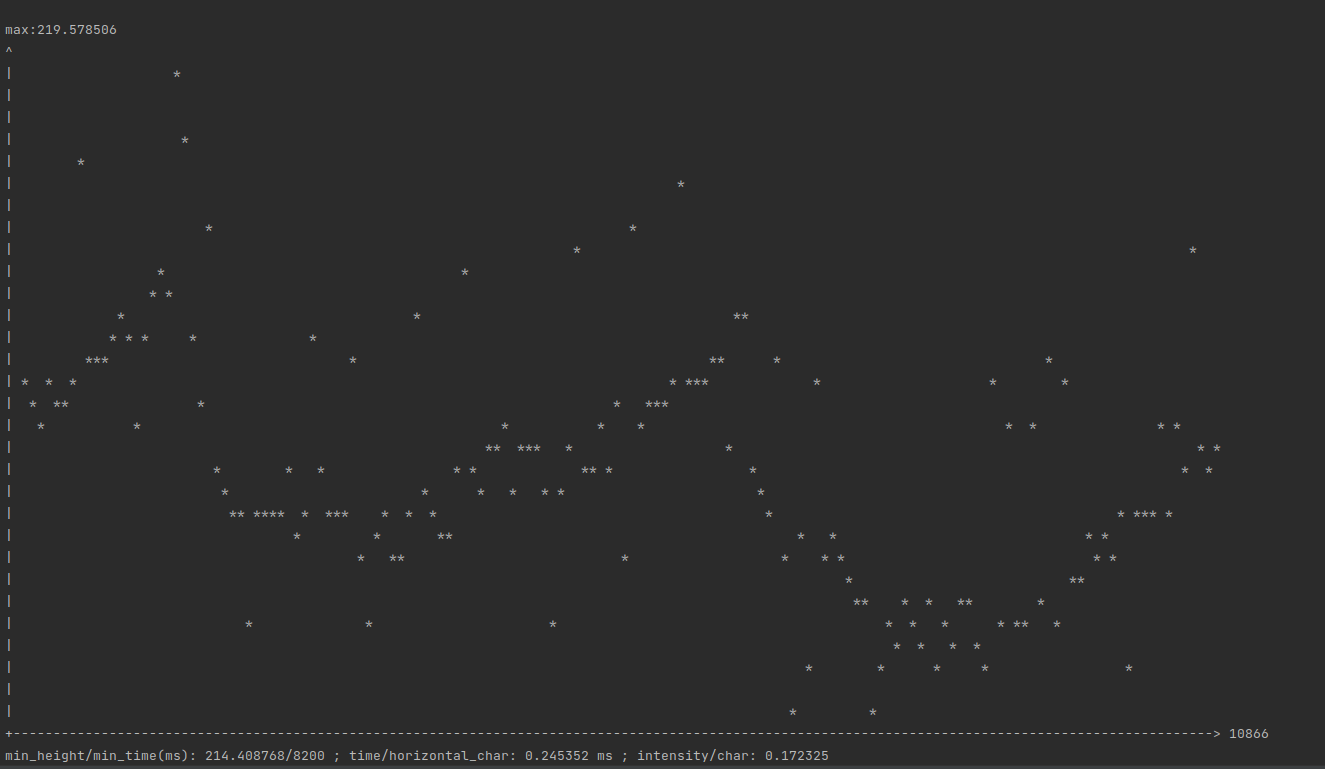
\includegraphics[width=\textwidth]{rawdata}
  \caption{Gráfico com as intensidades ao longo do tempo.}
  \label{fig:rawdata}
\end{figure}

\subsection{Normalização do gráfico}
\label{sec:normalizacao}
Como se pode observar, o gráfico obtido era difícil de analisar. Então, decidiu-se fazer um simples algoritmo de normalização, em que cada ponto seria a média dos últimos 10 pontos. Desta forma conseguiu-se um gráfico melhorado, apresentado na \cref{fig:normalized}.


\begin{figure}[H]
  \centering
  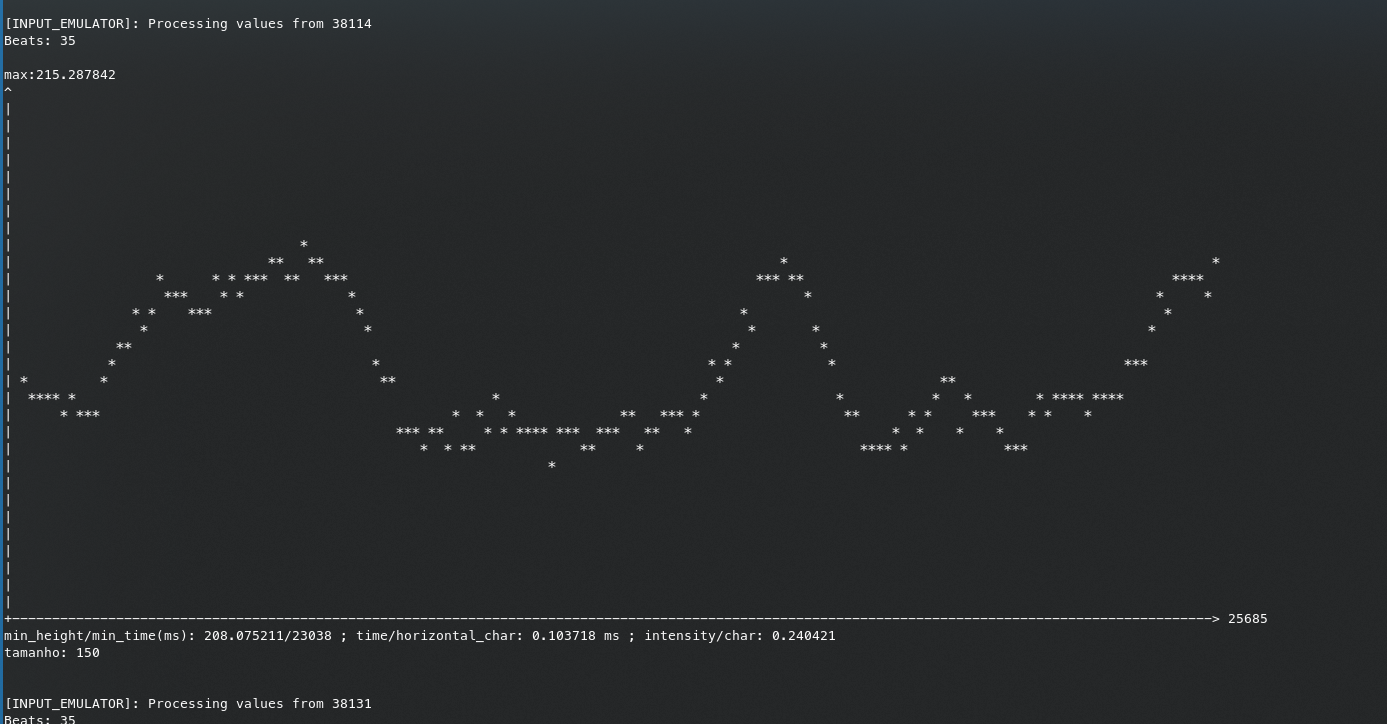
\includegraphics[width=\textwidth]{normalized}
  \caption{Gráfico com as intensidades normalizadas.}
  \label{fig:normalized}
\end{figure}

Com este simples método de normalização conseguem-se gráficos mais fáceis de analisar, cada vez maior for o número de pontos na media menos pontos existem que saltam tanto mas mais tempo demora a ter se valores usáveis e cada vez mais o gráfico fica com picos mais suaves, o que torna mais difícil descobrir as zonas de picos.


\subsection{Deteção de ciclos}
\label{sec:ciclos}
Um ciclo neste contexto consiste na passagem por um mínimo no gráfico, passando por um máximo e finalizando com um mínimo novamente,isto é considerado em termos práticos um batimento.

Concluindo, para calcular os batimentos por minuto faz-se a média das durações dos últimos ciclos.

\section{Testes}

\begin{wrapfigure}{r}[1cm]{2cm}
  \centering
  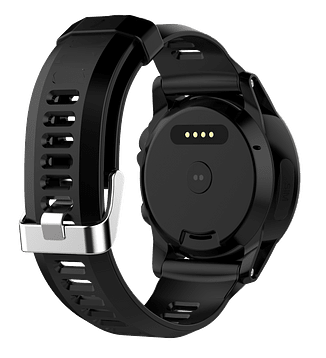
\includegraphics[height=2cm]{smartwatch.png}
  \caption{\textit{Smartwatch} com \acrshort{ir} \cite{smartwatch}}
  \label{fig:smartwatch}
\end{wrapfigure}

A biblioteca foi testada com uma pequena amostra de pessoas.
A amostra era de 5 pessoas, 2 crianças e 3 adultos. O sensor conseguia detetar o batimento, pelo polegar da amostra completa.

Comparou se os valores obtidos com o que o sensor de batimentos de um \textit{smartwatch} (\cref{fig:smartwatch}) em que se concluiu que o algoritmo desenvolvido obtinha valores inferiores ao do relógio ao redor de 10 a 20 batimentos por segundo.

A vantagem do algoritmo desenvolvido é ter um tempo de resposta a mudanças de batimento muito mais rápida o que é favorável para o jogo a ser desenvolvido.

\section{Conclusão}

A biblioteca não reporta números fiáveis para uma
deteção precisa dos batimentos por minuto de uma pessoa que a usa. Porém, serve perfeitamente para saber quando o batimento sobe ou desce, o que pode ser muito bem utilizado num jogo, principalmente para o \textit{DMS}.

Concluído este projeto, o estagiário ganhou experiência com a \gls{switch} e ganhou conhecimentos sobre o seu funcionamento e regras de utilização.

